Adicionalmente aos objetivos desta dissertação foi realizada a migração de \acrshort{http} para \acrshort{https} da plataforma da \acrshort{clav}.

Para tal, foi inicialmente investigado o \acrfull{ca} gratuito \textit{Let's Encrypt} por forma a usá-lo para obter certificados para ativar o \acrshort{https} nos websites (\acrshort{api} e interface) da plataforma \acrshort{clav}.

Na secção da solução apresenta-se os requisitos para esta migração bem como a arquitetura a desenvolver para obter uma plataforma com \acrshort{https}. 

Por fim, na secção da implementação descreve-se os passos realizados, aprofundando a configuração do \textit{Nginx} com várias recomendações de segurança para atingir a arquitetura apresentada na solução cumprindo os requisitos enunciados.

\section{Estado da Arte}

\subsection{Let's Encrypt}

Para ativar o \acrshort{https} num website ou numa \acrshort{api}, ou seja num domínio, é necessário um \acrfull{ca} de onde obter os certificados.

Para o caso da \acrshort{clav} necessita-se de um \acrshort{ca} gratuito e onde seja possível gerar certificados \acrfull{dv} (garantem apenas a validade do domínio e da informação trocada entre utilizador e domínio~\cite{certsTypes}).

Assim, a escolha recaiu no \textit{Let's Encrypt}, um dos \acrshort{ca}'s mais populares. O \textit{Let's Encrypt} foi criado pela \textit{Linux Foundation} é gratuito e \textit{open-source}. Além disso, tem como patrocinadores/doadores empresas como a \textit{Mozilla}, a \textit{Cisco}, o \textit{Google Chrome}, o \textit{Facebook}, entre outros. 

Para gerar/renovar o certificado \acrshort{dv} é necessário demonstrar que se possui o controlo sobre o domínio. Com o \textit{Let's Encrypt} isto é efetuado através do uso do protocolo \acrfull{acme} que necessita que se corra um agente de gestão de certificados (cliente \acrshort{acme}) no servidor do domínio a gerar o certificado. Assim é possível gerar/renovar certificados automaticamente sem a intervenção humana. Esta automatização é importante porque os certificados do \textit{Let's Encrypt} têm apenas a validade de 3 meses pelo que, se fosse necessário fazer manualmente teria de ser feito pelo menos de 3 em 3 meses.

A escolha do cliente \acrshort{acme} a usar irá depender se se tem acesso à \textit{shell} da máquina do servidor. Em caso afirmativo o \textit{Let's Encrypt} recomenda o uso do cliente \textit{Certbot}~\cite{letEnc}.

Caso não se tenha acesso à \textit{shell} irá depender se o provedor de \textit{hosting} suporta o \textit{Let's Encrypt} ou não. Se suportar então é fácil obter o certificado através do provedor. Caso contrário, pode-se pedir ao provedor o suporte (que não resolve de imediato o problema nem é de resolução garantida) ou se o provedor permitir o \textit{uploud} de certificados é possível através do \textit{Certbot} gerar um certificado em modo manual mas que acarreta efetuar esta tarefa pelo menos de 3 em 3 meses para renovar o certificado pelo que não é recomendado.

Uma pequena chamada de atenção, o \textit{Let's Encrypt} possui \textit{Rate Limits}~\cite{LErateLimits} pelo que num ambiente de testes deve ser usado o ambiente de testes do \textit{Let's Encrypt}\footnote{Ver \url{https://letsencrypt.org/docs/staging-environment/}} e não o de produção.

\subsubsection{Validação do Domínio}\label{sec:valDom}

Nesta secção será explicado como é realizada a validação do domínio para a geração/renovação/revogação dos certificados.

Na primeira vez que o agente (cliente \acrshort{acme}) interage com o \textit{Let's Encrypt} gera um novo par de chaves e prova ao \textit{Let's Encrypt} que o servidor controla um ou mais domínios.~\cite{domainValidation}

Para iniciar o processo de validação, o cliente \acrshort{acme} questiona o \textit{Let's Encrypt} para que lhe indique o que necessita fazer para provar que controla o domínio~\cite{domainValidation}. Assuma-se que queremos validar o domínio \texttt{example.com}.
O \textit{Let's Encrypt} irá gerar um ou mais conjuntos de desafios após olhar para o nome do domínio.

Há duas formas (desafios) do cliente \acrshort{acme} provar que controla o domínio perante o \textit{Let's Encrypt}~\cite{domainValidation}:
\begin{itemize}
    \item Providenciar um \acrshort{dns} \textit{record} sobre \texttt{example.com}
    \item Providenciar um recurso \acrshort{http} num \acrshort{uri} conhecido em \texttt{http://example.com/} (é colocado normalmente em \texttt{http://example.com/.well-known/acme-challenge})
\end{itemize}

Juntamente com os desafios, o \textit{Let's Encrypt} envia um \textit{nonce} (\textit{string} usada uma única vez) que o cliente deve assinar com a chave privada por forma a garantir que este controla o par de chaves evitando \textit{replay attacks}\footnote{Para mais informação ver \url{https://www.kaspersky.com/resource-center/definitions/replay-attack}}.

Veja-se agora, na figura~\ref{fig:domainValidation}, um exemplo concreto em que o cliente \acrshort{acme} usa o segundo desafio para provar que controla o domínio (\texttt{example.com}):

\begin{figure}[H]
    \centering
    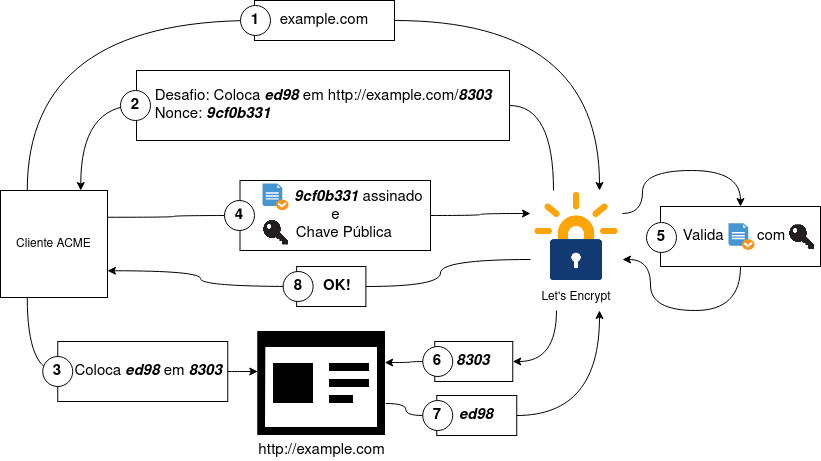
\includegraphics[width=1\textwidth]{img/domainValidation.png}
    \caption{Exemplo de validação do domínio pelo \textit{Let's Encrypt} com sucesso\label{fig:domainValidation}}
\end{figure}

Como o desafio teve sucesso e o \textit{nonce} assinado pelo cliente \acrshort{acme} é válido então o cliente \acrshort{acme} identificado pela chave pública está autorizado a gerir os certificados para o domínio \texttt{example.com}. Assim, para gerar/renovar/revogar o certificado para o domínio basta enviar mensagens de gestão do certificado assinadas com o chave privada (a que assinou o \textit{nonce}) para o \textit{Let's Encrypt}.

\subsubsection{Cliente \textit{acme.sh}}\label{sec:soaACMEsh}
Apesar do cliente recomendado pelo \textit{Let's Encrypt} ser o \textit{Certbot} este necessita de ter permissões \textit{root} bem como tem várias dependências para ser executado. Já o cliente \textit{acme.sh}\footnote{Ver \url{https://github.com/acmesh-official/acme.sh}} é uma \textit{script} \textit{bash} que para a sua instalação basta efetuar \textit{download} da \textit{script} deste. Além disso, não necessita de quaisquer dependências nem de acesso \textit{root} (apenas necessita em casos especiais). A sua utilização, tal como o \textit{Certbot}, é feita através da execução de comandos \textit{bash}.

Para instalar basta:
\begin{verbatim}
curl https://get.acme.sh | sh
#ou
wget -O -  https://get.acme.sh | sh
\end{verbatim}

Esta instalação irá ativar desde logo a auto renovação dos certificados através da criação de um \textit{cron job}\footnote{Mais informação em \url{https://www.ostechnix.com/a-beginners-guide-to-cron-jobs/}} pelo que o cliente \textit{acme.sh} irá correr periodicamente para verificar e renovar os certificados se necessário.

Para obter um certificado executa-se:
\begin{verbatim}
acme.sh --issue -d <dominio> -w <pasta web root>
\end{verbatim}

Após obter o certificado, este pode ser instalado no \textit{Nginx} com:
\begin{verbatim}
acme.sh --install-cert -d example.com \
    --key-file /path/to/keyfile/in/nginx/key.pem  \
    --fullchain-file /path/to/fullchain/nginx/fullchain.pem \
    --reloadcmd "nginx -s reload"
\end{verbatim}

Neste último comando, o ficheiro de configuração do \textit{Nginx} tem de estar à espera que os ficheiros do certificado estejam em \path{/path/to/keyfile/in/nginx/key.pem} e em \path{/path/to/fullchain/nginx/fullchain.pem}.

\section{Solução}

O \acrfull{http} possui várias vulnerabilidades de segurança entre as quais \textit{man-in-the-middle attack}\footnote{Ver \url{https://owasp.org/www-community/attacks/Man-in-the-middle_attack}} bem como a possibilidade de \textit{eavesdropping}\footnote{Ato de ouvir de forma secreta ou furtiva conversas ou comunicações particulares de outras pessoas sem o consentimento destas} e \textit{tampering}\footnote{Alteração deliberada ou adulteração dos dados enviados entre cliente e servidor} da comunicação entre cliente e servidor.

Com o intuito principal de superar estas vulnerabilidades foi criada a extensão ao \acrshort{http} o \acrfull{https}. Este protocolo de comunicação é encriptado através do uso de \acrfull{tls} ou através do uso do já \textit{deprecated}, por razões de segurança, \acrfull{ssl}. O \acrshort{https} oferece autenticação dos \textit{websites} acedidos bem como privacidade e integridade dos dados trocados.

É assim de extrema importância a migração do atual \acrshort{http} para \acrshort{https} tanto na \acrshort{api} da \acrshort{clav} bem como na interface da \acrshort{clav}.

Por forma a realizar esta migração há um conjunto de requisitos a cumprir:\label{sec:sol_httpsReq}
\begin{itemize}
    \item Usar um \acrshort{ca} gratuito
    \item Os certificados devem ser renovados automaticamente
    \item Permitir criar uma \textit{script} de automatização para o \textit{deployment}
    \item Possuir as seguintes recomendações de segurança:
    \begin{itemize}
        \item Redirecionar os pedidos \acrshort{http} para \acrshort{https} por forma a impedir que os utilizadores usem uma conexão insegura bem como evitar que alguém se faça passar pela \acrshort{clav} em \acrshort{http}
        \item Adicionar o cabeçalho \acrshort{hsts} recomendado~\cite{hsts,hsts2}
        \item Adicionar vários cabeçalhos e configurar o \textit{reverse proxy} por forma a tornar o \acrshort{https} mais forte e a \acrshort{api}/interface mais segura. Ver~\cite{helmet,letEnA+,dhparams,secExpress,strongSSL}
        \item Adicionar o cabeçalho \acrfull{csp}~\cite{helmetCSP,csp}
    \end{itemize}
\end{itemize}


Para realizar esta migração a primeira decisão a tomar é o \acrfull{ca} de onde iremos comprar/obter os certificados. Existem vários \acrshort{ca}s mas visto termos a restrição de que este deve ser gratuito apenas nos sobra uma alternativa bastante popular, o \textit{Let's Encrypt}. O único revês de usar o \textit{Let's Encrypt} é o facto de que os certificados tem uma validade de apenas 90 dias.

Após se decidir que será usado o \acrshort{ca} \textit{Let's Encrypt} é necessário decidir que cliente \textit{Let's Encrypt} usar. Este cliente permite a obtenção e renovação de certificados. Existem vários clientes\footnote{Ver \url{https://letsencrypt.org/docs/client-options/}} dos quais o \textit{Let's Encrypt} recomenda o \textit{Certbot}\footnote{Ver \url{https://certbot.eff.org/}}. Contudo para usar \textit{Certbot} é necessário ter permissões \texttt{root} (\texttt{sudo}) no servidor bem como é necessário instalar algumas dependências. Por tais razões foi usado o \texttt{acme.sh} (Ver~\ref{sec:soaACMEsh}). O \texttt{acme.sh} é quem irá tratar de toda a gestão dos certificados, renovando-os quando necessário (a renovação é feita a cada 60 dias).

Tendo em conta os requisitos a solução passa por colocar um \textit{reverse proxy} em \textit{Nginx} à frente da \acrshort{api} de dados, algo que já não é necessário na interface visto este (\textit{Nginx}) já estar presente. Após isso, a solução passará por configurar o \textit{Nginx}, tanto na \acrshort{api} de dados como na interface, com as várias recomendações de segurança. Passa também por automatizar o \textit{deployment} através de \textit{Docker} e \textit{Docker-Compose} bem como a criação de algumas pequenas \textit{scripts} para:
\begin{itemize}
    \item gerar certificado local autoassinado com o único objetivo de permitir o primeiro inicio do \textit{Nginx} (ainda não foram gerados os certificados dos domínios) para ser possível o \texttt{Let's Encrypt} validar o controlo sobre o domínio (ver~\ref{sec:valDom}) permitindo a geração dos certificados necessários
    \item automatizar a instalação do cliente \acrshort{acme} \texttt{acme.sh} (\textit{download} e instalação)
    \item gerar o primeiro certificado para os domínio(s) pretendido(s) com o \texttt{acme.sh}
    \item instalar o primeiro certificado no caminho apropriado com o \texttt{acme.sh} de onde o \textit{reverse proxy} o irá obter
    \item gerar \textit{\acrshort{dh} parameters} mais fortes para a troca de chaves com recurso ao \textit{OpenSSL}
    \item instalar dependências no \textit{container} onde se encontra o \textit{Nginx}:
    \begin{itemize}
        \item \texttt{openssl} para a geração de um certificado local autoassinado e dos \acrshort{dh} \textit{paremeters}
        \item \texttt{cron} para o \texttt{acme.sh} criar um \textit{cron job} diário para a verificação/renovação do certificado
        \item \texttt{curl} para fazer \textit{download} do \texttt{acme.sh}
    \end{itemize}
\end{itemize}

A arquitetura a desenvolver com \acrshort{https}, presente na figura~\ref{fig:apiHttpsArch}, é semelhante à presente na figura~\ref{fig:clav_struct2} tendo como única diferença a adição do \textit{Nginx} à frente da \acrshort{api} de dados:
\begin{figure}[H]
    \centering
    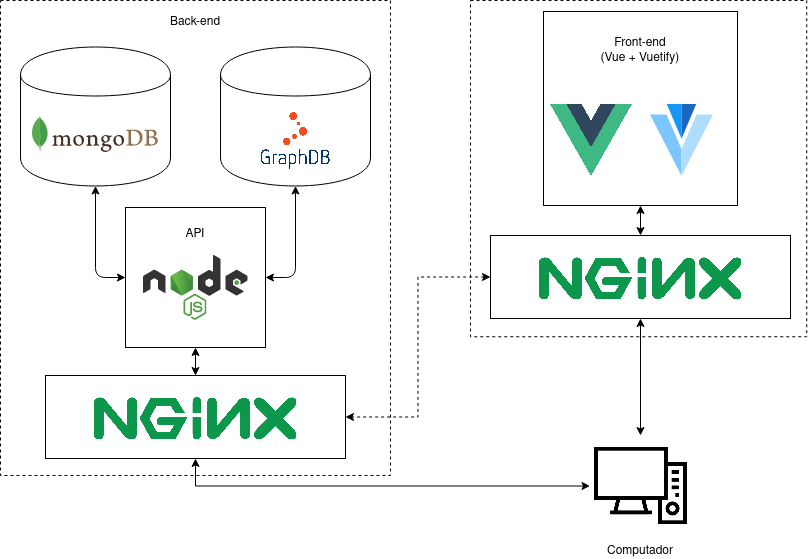
\includegraphics[width=0.9\textwidth]{img/apiHttpsArch.png}
    \caption{Arquitetura a desenvolver com \acrshort{https}\label{fig:apiHttpsArch}}
\end{figure}

A ligação a tracejado entre os dois \textit{Nginx}'s pode ou não existir, irá depender se se pretende ou não que o servidor da interface reencaminhe pedidos para o servidor da \acrshort{api} de dados.

\section{Implementação}

A partir dos requisitos já enunciados em~\ref{sec:sol_httpsReq} foram criadas duas \textit{scripts} uma para correr antes de iniciar o \textit{Nginx} e outra para correr depois de o \textit{Nginx} iniciar.

A \textit{script} que corre antes de iniciar o \textit{Nginx} instala o \texttt{openssl}, gera o certificado autoassinado e \acrshort{dh} \textit{parameters} para permitir o \textit{boot} do \textit{Nginx}.

Já a \textit{script} que corre após o inicio do \textit{Nginx} realiza o \textit{download} do \texttt{acme.sh}, instala-o, obtém o primeiro certificado para o(s) domínio(s) com o \texttt{acme.sh}, instala o certificado com o \texttt{acme.sh}, gera \acrshort{dh} \textit{parameters} mais fortes e, por fim, reinicia o \textit{Nginx} para que o novo certificado e \acrshort{dh} \textit{parameters} tenham efeito, ou seja, sejam usados pelo \textit{Nginx}.

Quanto à configuração do \textit{Nginx} entre a da \acrshort{api} de dados e a da interface há poucas diferenças. Estas diferenças são que na configuração \textit{Nginx} na \acrshort{api} de dados é encaminhado os pedidos para o servidor em \textit{Node.js} enquanto que na configuração \textit{Nginx} da interface há duas variantes onde só uma é usada:
\begin{itemize}
    \item Apenas serve os ficheiros estáticos da interface
    \item Serve os ficheiros estáticos da interface e reencaminha os pedidos para a \acrshort{api} de dados, aqueles em que o caminho começa em \texttt{/<versão\_api>/} ou é igual a \texttt{/clav.yaml}.
\end{itemize}

Quanto às configurações comuns estas serão apresentadas de seguida, explicando para que servem.

Para cumprir o requisito de redirecionamento dos pedidos de \acrshort{http} para \acrshort{https} é colocado o seguinte bloco de código na configuração:
\begin{lstlisting}[caption=Redirecionamento de \acrshort{http} para \acrshort{https} e validação do domínio na configuração \textit{Nginx}]
  server {
    listen <Porta HTTP>;
    server_name localhost;

    location /.well-known/acme-challenge/ {
      alias /var/www/html/.well-known/acme-challenge/;
    }

    location / {
      return 301 https://$host$request_uri;
    }
  }
\end{lstlisting}
Além disso, permite a validação do controlo do domínio por parte do \textit{Let's Encrypt} visto que este pequeno excerto permite que o \textit{Nginx} receba pedidos em \path{/.well-known/acme-challenge/}, caminho este onde é colocado a resposta de um desafio do \textit{Let's Encrypt}.

Fica assim definido o que se faz quando se recebe um pedido \acrshort{http}. Para os pedidos \acrshort{https} é criado também um bloco \texttt{server} onde é ativado o \acrshort{http}2 e é indicado os ficheiros com o certificado:
\begin{lstlisting}[caption=Certificado na configuração \textit{Nginx}]
  server {
    listen <Porta HTTPS> ssl http2;
    server_name localhost;

    ssl_certificate $CERTS/fullchain.pem;
    ssl_certificate_key $CERTS/key.pem;
    ...
  }
\end{lstlisting}
Depois são adicionadas várias configurações recomendadas~\cite{helmet,letEnA+,dhparams,secExpress,strongSSL,helmetCSP,csp,hsts,hsts2}:
\begin{lstlisting}[caption=Recomendações de segurança na configuração \textit{Nginx}]
  server {
    ...

    #Protocolos SSL permitidos
    ssl_protocols TLSv1.2 TLSv1.3;

    #Ciphers SSL permitidos a usar por ordem de preferência
    ssl_ciphers "EECDH+AESGCM:EDH+AESGCM:ECDHE-RSA-AES128-GCM-SHA256:AES256+EECDH:DHE-RSA-AES128-GCM-SHA256:AES256+EDH:ECDHE-RSA-AES256-GCM-SHA384:DHE-RSA-AES256-GCM-SHA384:ECDHE-RSA-AES256-SHA384:ECDHE-RSA-AES128-SHA256:ECDHE-RSA-AES256-SHA:ECDHE-RSA-AES128-SHA:DHE-RSA-AES256-SHA256:DHE-RSA-AES128-SHA256:DHE-RSA-AES256-SHA:DHE-RSA-AES128-SHA:ECDHE-RSA-DES-CBC3-SHA:EDH-RSA-DES-CBC3-SHA:AES256-GCM-SHA384:AES128-GCM-SHA256:AES256-SHA256:AES128-SHA256:AES256-SHA:AES128-SHA:DES-CBC3-SHA:HIGH:!aNULL:!eNULL:!EXPORT:!DES:!MD5:!PSK:!RC4";

    #DH parameters mais forte
    ssl_dhparam $CERTS/dhparam.pem;
    #Especifica a curva a usar para os ciphers ECDHE
    ssl_ecdh_curve secp384r1;

    #Ativa stapling
    ssl_stapling on;
    ssl_stapling_verify on;

    #Melhora tolerância quando o endereço de um domínio muda
    resolver 8.8.8.8 8.8.4.4 valid=300s;
    resolver_timeout 5s;

    #Adição de cabeçalhos que melhoram a segurança
    add_header Strict-Transport-Security "max-age=31536000; includeSubDomains; preload";
    add_header X-DNS-Prefetch-Control off;
    add_header X-Frame-Options SAMEORIGIN;
    add_header X-Download-Options noopen;
    add_header X-Content-Type-Options nosniff;
    add_header X-XSS-Protection "1; mode=block";
    add_header Content-Security-Policy <Cabeçalho CSP>;
  }
\end{lstlisting}
O valor do cabeçalho \texttt{Content-Security-Policy} varia de acordo se for para a \acrshort{api} de dados ou para a interface. A adição dos cabeçalhos na \acrshort{api} de dados é feita pelo \texttt{helmet} (Ver~\cite{helmet}) no servidor \textit{Node.js} em vez de ser no \textit{Nginx} mas o resultado final é igual ao uso desta configuração.

Por fim, na configuração do \textit{Nginx} é também adicionado fora dos \texttt{servers} a diretiva 
\begin{verbatim}
ssl_prefer_server_ciphers on;
\end{verbatim}
com o objetivo de indicar a preferência de uso dos \textit{ciphers} \acrshort{ssl} do servidor definida na configuração (diretiva \texttt{ssl\_ciphers}) em vez dos \textit{ciphers} do cliente. Ficam assim cumpridas todas as recomendações de segurança e os requisitos apresentados em~\ref{sec:sol_httpsReq}, sendo usado para o \textit{deployment} o \textit{docker} e o \textit{docker-compose}. O \textit{deployment} é explicado mais à frente na secção~\ref{sec:deployNoKong}.
